% **************************************************
%   Wichtig für die verwendung der hsrmreport-Klasse!
%   
%   Die Datei hsrmreport.cls muss in dem selben Ordner sein
%   wie die .tex Datei die diese Klasse verwenden möchte.
%
%   Desweiteren ist die Dokumentenklasse nach aktuellem 
%   noch ohnen Optionen, sprich Zweiseitig, änderung 
%   der Schriftgröße oder ähnliches. Ich werde versuchen 
%   diese Features hinzu zufügen sobald es mir möglich ist. 
%
%   Falls Ihr Probleme, Anregungen oder Verbesserungen habt,
%   könnt ihr mir das gerne mitteilenen.
%
%   Es kann sein das ihr evtl. manche Packete noch installieren 
%   müsst bevor die Klasse Fehlerfrei funktioniert.
%   Meldungen wie "Command terminated with space." können ignoriert werden.
%
%   Ich werde auch eine Übersicht aller Pakete schreiben, die ich verwendet habe.
%      
%
%   E-Mail: timjonas.wechler@student.hs-rm.de
% **************************************************


\documentclass[printbib]{hsrmreport}
% **************************************************
% Ihr könnte die Angaben der TITELSEITE hier ändern
% **************************************************
\newcommand{\titel}{Resistives Touch-Panel}
\newcommand{\studiengang}{Angewandte Physik}
\newcommand{\studienrichtung}{Physikalische Technik}
\newcommand{\dokumentenart}{Laborbericht}
\newcommand{\kurs}{LV:\ Embeeded System Labor}
\newcommand{\versuchsdurchfuehrungDatum}{4. Februrar 2022}
\newcommand{\AbgabeOrt}{Rüsselsheim am Main}

%Falls ihr weniger als vier Studenten seit könnt ihr dies Einträge die zu viel sind einfach löschen. 
%Ein Feature für das angeben der Mat.Nr. ist noch in Arbeit. 
\newcommand{\studentA}{Dennis Hunter}
\newcommand{\matStudentA}{()}
\newcommand{\studentB}{Tim-Jonas Wechler}
\newcommand{\matStudentB}{(1137877)}
\newcommand{\studentC}{}
\newcommand{\matStudentC}{}
\newcommand{\studentD}{}
\newcommand{\matStudentD}{}

\newcommand{\Referent}{}
\newcommand{\Korreferent}{}


\usepackage{datatool}



% Mit dem Befehl \today wird immer das aktuelle Datum auf der Titelseite ausgebeben.
% Wenn dies nicht erwünscht ist einfach manuell das gewünschte Datum eintragen.
\newcommand{\datum}{\today}



\begin{document}
    % **************************************************
    %
    % HIER BEGINNT DER BERICHT
    %
    % **************************************************

    \chapter{Einleitung}
Seit einigen Jahren findet man immer häufiger Bedienungen mit Touchscreens.
Ihr Einsatzbereich scheint keine Grenzen zu haben und so hat sich die Technologie in den letzten Jahren rasant weiterentwickelt.


\section{Ziel des Projekts}
In dieser Projektarbeit ist es Ziel, die Aufnahme und Auswertung der Koordinaten mittels eines resistiven Touchscreen.
Zum Schluss soll die Steuerung noch dahingehend erweitert werden, dass damit die Maus eines PC's gesteuert wird.


\section{Grundlagen}
\subsection{Resistives Touchscreen}
Es gibt bei den resistiven Touchscreens zwei unterschiedliche Gruppen.
Zum einen gibt es 4-Wire resistive Touchscreens.
Diese haben vier Anschlüsse, über die die Positionsauswertung läuft.
Zudem gibt es noch die 5-Wire resistive Touchscreens.
Hier sind fünf Anschlüsse, über die die Positionsauswertung durchgeführt wird.

Bei einem 4-Wire resistiven Touchscreen gibt es zwei Ebenen, bei denen die obere auf die untere gedrückt werden kann.
Eine Ebene ist mit Elektronen geladen und über die andere Ebene misst man die Spannung die in eine Richtung bei der Berührung abfällt.
Für die andere Richtung ist es gespiegelt.
Die Ebene, die die Spannung in eine Richtung misst, ist für die andere Richtung mit Elektronen geladen.
Die Messung wird dann von der anderen Ebene durchgeführt.
Über die unterschiedlichen Beträge der Spannung lässt sich dann die Koordinate in x-Richtung und y-Richtung bestimmen.

Die 5-Wire resistive Touchscreens haben ebenfalls zwei Ebene.
Der Unterschied zu den 4-Wire Touchscreen liegt darin, dass es nur eine Ebene gibt, die geladen ist.
Normalerweise ist es die untere Schicht.
Die obere Schicht misst  für x-Richtung und y-Richtung die abfallende Spannung.
Auch hier wird durch Druck auf die obere Schicht ein Kontakt zwischen den beiden Ebenen erstellt, damit die Messung durchgeführt werden kann.

Die 5-Wire Touchscreens sind gegenüber den 4-Wire Widerstandsfähiger und haben dadurch eine längere Lebenserwartung.\cite{5w4w}

In diesem Projekt wird ein 4-Wire resistiver Touchscreen verwendet von der Firma Fujitsu verwendet.

Der verwendete Touchscreen besitzt für jede Richtung (x und y) jeweils zwei Anschlüsse \cref{fig:4w}.
In x, wie auch in y-Richtung sind jeweils 2 Widerstände eingezeichnet.
Diese sollen den Widerstand auf der jeweiligen Ebene, über die die Spannung abfällt, darstellen.
Die Ströme wie auch die Widerstände bewegen sich hierbei in einem niedrigen Wertebereich.
Die Aufnahme der Werte für einen Koordinatenwert wird über das Prinzip des Spannungsteiler realisiert.
\begin{figure}
    \centering
    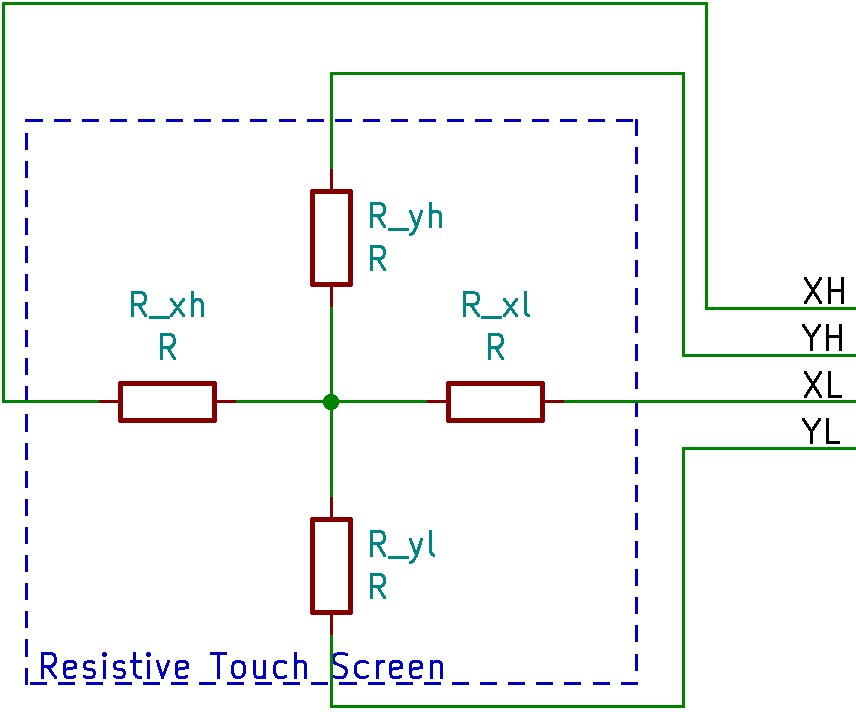
\includegraphics[width=0.6\linewidth]{fig/4-wire.jpg}
    \caption{Schemadarstellung eines 4-Wire resistiven Touchscreen}
    \label{fig:4w}
\end{figure}
\subsection{Arduino Leonardo Board}
Im Labor wurde hauptsächlich das Arduino Uno Board verwendet.
Die Unterschiede zwischen diesen beiden liegen darin, dass das Leonardo Board die Möglichkeit hat, sich als Peripherie an einem PC an zu melden.
Ermöglicht wird dies durch den Mikrocontroller ATmega32u4.
Der Mikrocontroller arbeitet nicht mit einem USB-Chip, sonder verarbeitet intern die serielle eingehende Daten und konvertiert diese für die Nutzung der USB-Schnittstelle.


    \chapter{Versuchsaufbau}    
Das Porjekt wird fertig zusammengebaut ausgehändigt.
\begin{figure}[ht!]
    \centering
    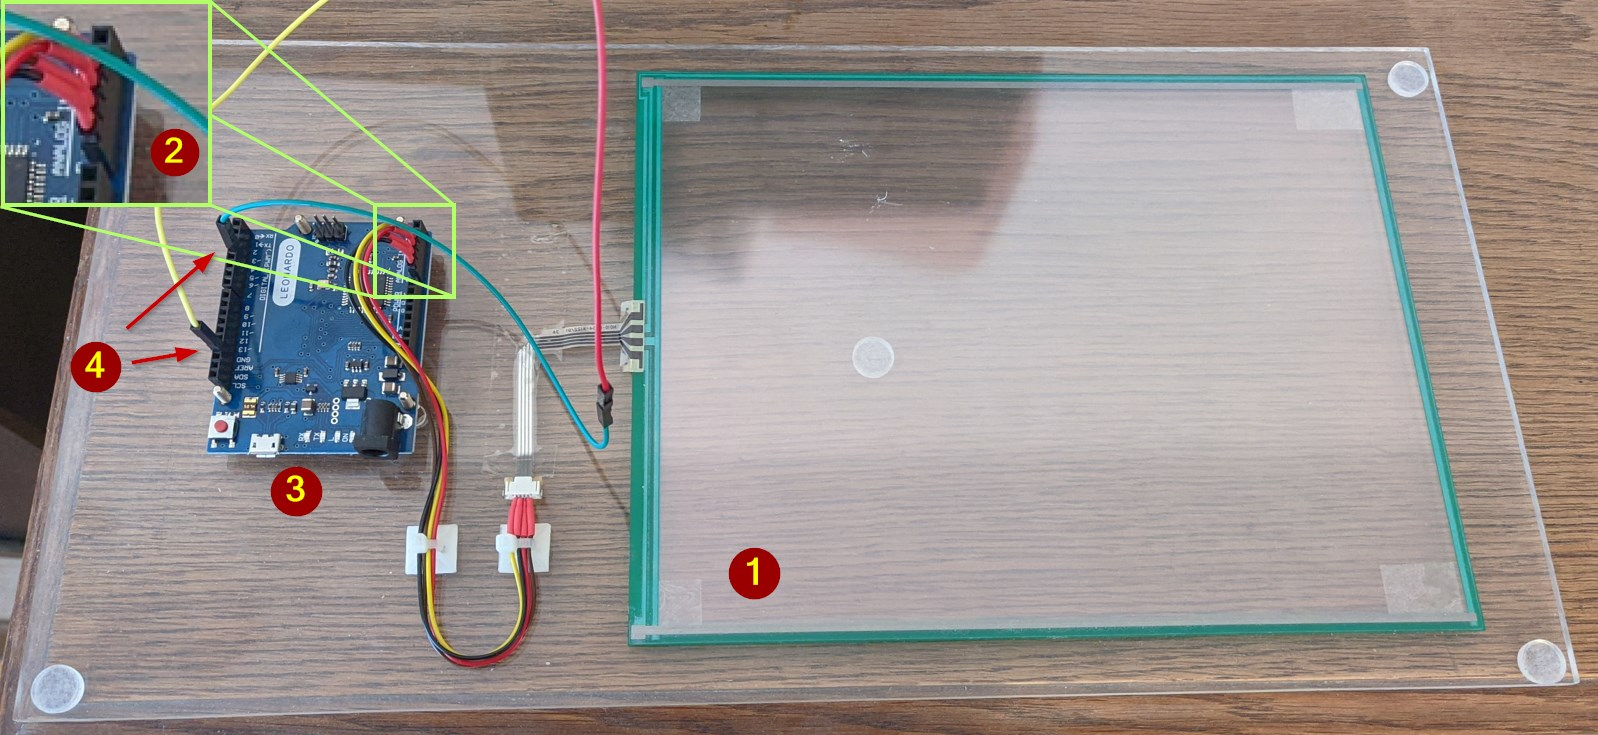
\includegraphics[width=\linewidth]{fig/aufbau_annotated.jpg}
    \caption{Versuchsaufbau}
    \label{fig:aufbau}
\end{figure}
\begin{itemize}
    \item[1] Touchscreen
    \item[2] Anschlüsse des Touchscreen am Leonardo Board
    \item[3] Arduino Leonardo
    \item[4] Pins für die Steuerung, ob man die Maus bedienen möchte oder nicht
\end{itemize}
    \chapter{Aufnahme von Koordinatenpunkte}
\section{Problem}
Wenn ein Koordinatenpunkt aufgenommen werden will, gibt es mehrere Probleme auf die man stößt.

Zum einen kann nicht gleichzeitig die X und Y Komponente der Koordinate bestimmt werden. Dies muss nacheinander folgen.
Grund hierfür ist dem Aufbau des Touchscreens geschuldet.

Bei der Inbetriebnahme wird sich noch ein weiteres Problem ergeben.
Falls der Touchscreen nicht betätigt wird, gibt der Mikrocontroller trotzdem Werte aus.
Dabei handelt es sich um Werte die keinen Sinn ergeben und die Steuerung der Maus z.B. bei einer Ruhephase stören würden.

Bei einer Messreihe kann es vereinzelt zu einem Wertesprung kommen. 
Dieses Problem ist der Messunsicherheit des Systems geschuldet. 
Diese Sprünge gilt es aus der Messreihe heraus zu filter und zu glätten.

\section{Lösungsansatz}
Um das Problem, bei einer nicht Betätigung des Touchscreens, zu lösen, soll vor einer Aufnahme von Koordinatenwerte geprüft werden, ob der Touchscreen betätigt wird.
Ist dies der Fall so soll die Messung durchgeführt werden.

Um eine Koordinatenkomponente zu bestimmen, benötigt man drei Anschlüsse des Touchscreens.
Zwei davon sind in der Richtung die man messen möchte und der dritte Anschluss ist einer der beiden übrigen Anschlüsse.
Mit diesem wird der Spannungsteiler auf gespannt um den Wert der Koordinate zu bestimmen.

In den \cref{fig:xylesen} auf \cref{fig:xylesen} wird dieser Lösungsansatz veranschaulicht.
Bei dem Lesen der x-Komponente \cref{fig:xlesen} wird der Pin \verb$X_Le$ (steht für X-Links) auf eine Spannung von \SI{5}{V} gesetzt.
Der Pin \verb$X_Ri$ (steht für X-Rechts) wird auf \SI{0}{V} gezogen.
Der Pin  \verb$Y_Up$ (steht für Y-Oben) wird auf den Modus \verb$Hi Z$ (Hohe Eingangsimpedanz) gesetzt. In diesem Modus fällt der Widerstand in die y-Richtung so klein aus, das er vernachlässigbar gering ist.
Um die y-Komponente zu lesen wird das wie in \cref{fig:ylesen} auf \cpageref{fig:ylesen} der Pin \verb$Y_Up$ auf \SI{5}{V} gesetzt und der Pin \verb$Y_Lo$ (steht für Y-Unten) auf \SI{0}{V} gesetzt.
Hier wird der \verb$Hi Z$ Modus auf den Pin \verb$X_Le$ gesetzt.

Um nun noch eine Messunsicherheiten aus zu filtern sollen, bei der Messung einer Koordinatenkomponente, mehrere Messpunkte aufgenommen werden.
Diese werden anschließend über ein Filter-Funktion ausgewertet.
Der Wert der bei der Auswertung als Ergebnis herauskommt, wird als gemessene Koordinatenkomponente ausgegeben.
Das Schaltbild hierzu ist in \cref{fig:schaltbild} zu sehen.

\begin{figure}[ht!]
    \begin{subfigure}{0.49\textwidth}
        \centering
        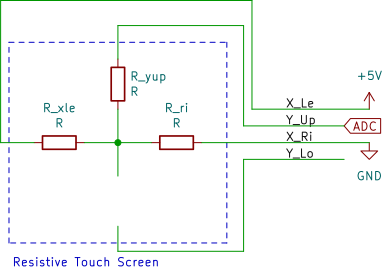
\includegraphics[width=\textwidth]{fig/xlesen.png}
        \caption{in x-Richtung}
        \label{fig:xlesen}
    \end{subfigure}
    \hfill
    \begin{subfigure}{0.49\textwidth}
        \centering
        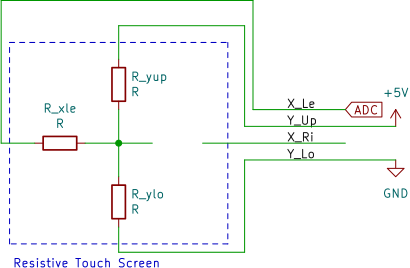
\includegraphics[width=\textwidth]{fig/ylesen.png}
        \caption{in y-Richtung}
        \label{fig:ylesen}
    \end{subfigure}
    \caption{Schaltbild für das Messen der Koordinatenpunkte}
    \label{fig:xylesen}
\end{figure}
\begin{figure}[ht!]
    \centering
    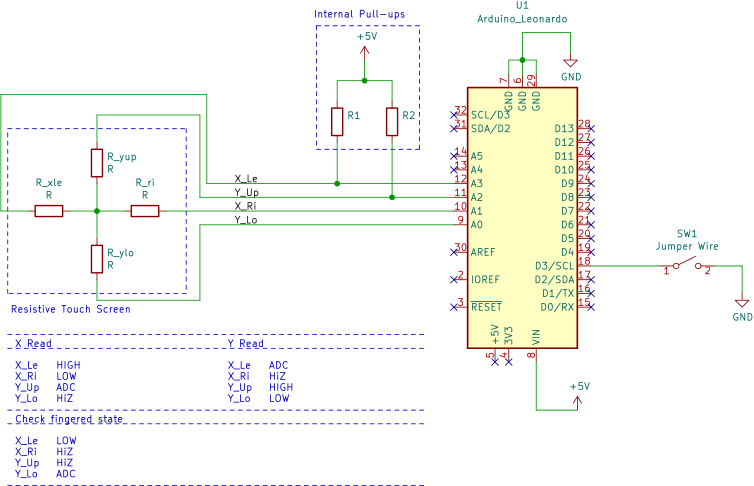
\includegraphics[width=\linewidth]{fig/schaltbild.png}
    \caption{Schaltbild des Projekts}
    \label{fig:schaltbild}
\end{figure}
Die einzelne Lösungsansätze werden in der Arduino-Umgebung umgesetzt.
Der Programmablauf ist in \cref{fig:flowchart} als Flow-Chart dargestellt.

\begin{figure}
    \centering
    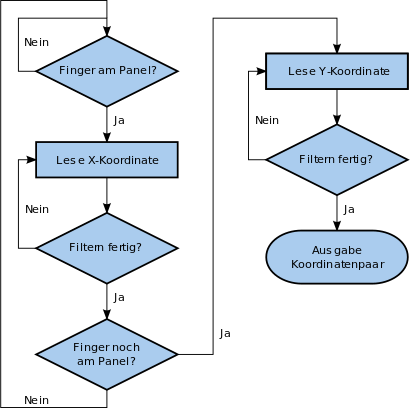
\includegraphics[scale=0.45]{fig/flow_chart.png}
    \caption{Darstellung des Programmablaufs}
    \label{fig:flowchart}
\end{figure}

    \chapter{Untersuchung der Messdaten}
Um eine Aussage über die Qualität des Touchscreen treffen zu können, werden mehrere Untersuchungen angestellt. 

Bei der ersten Untersuchung wurde auf die Mitte des Touchscreen gedrückt und die Position für eine gewisse Zeit gehalten.
Es wurden hierfür gefilterte und ungefilterte Messreihen erstellt (siehe Abschnitt \ref{ab:genau}).

Um die erste Untersuchung zu erweitern wurde die Mitte des Touchscreen, in der nächsten Untersuchung, wiederholt gedrückt. Hierbei ist die Wiederholbarkeit eines Punktes auf dem Touchscreen untersucht worden. 
Die Auswertung ist in Abschnitt \ref{ab:wiederholung} zu finden.

Bei der letzten Untersuchung wurde die Linearität des Touchscreen untersucht. Hierfür gibt der Hersteller eine Garantie, unter der sich die Linearität des Touchscreen befinden soll. 
Den Wert der angegeben wird liegt bei \SI{1,5}{\%} (siehe \ref{ds:touch} Seite 3 des Datenblatts). 

Um die Nachfolgende Untersuchungen korrekt durchführen zu können muss zu nächst der Reaktionsbereich des Touchscreens ermittelt werden.
Durch seine Bauform hat dies einen Randbereich an dem es nicht zuverlässig Werte ausgibt. Umkehrschluss, das Programm erkennt nicht das etwas den Touchscreen betätigt. 
Durch Untersuchungen des Randbereichs wurde in X-Richtung ein Arbeitsbereich von \SI{214,5}{mm} und in Y-Richtung eine Bereich von \SI{161,0}{mm} ermittelt.

Durch Ausprobieren wurden die maximal und minimal ADC-Werte in die jeweilige Richtung ebenfalls ermittelt. 
\begin{table}[ht!]
    \caption{maximal und minimal ADC-Werte}
    \begin{center}
        \begin{tabular}{ c |c| c }
                & x-Richtung & y-Richtung \\ \hline
         max. ADC-Werte & 961 & 917 \\  \hline
         min. ADC-Werte& 68 & 108 \\   
        \end{tabular}
    \end{center}   
\end{table}

Mit diesen Werten lässt sich Arbeitsbereich (in ADC-Werten) des Touchscreen in jede Richtung bestimmen.
\begin{align}
    ADC_{x,len} &= 1024 - 68 -(1024-961)\nonumber\\
    ADC_{x,len} &= 893\label{eq:adcxlen}\\
    ADC_{y,len} &= 1024-108-(1024-917)\nonumber\\
    ADC_{y,len} &= 809\label{eq:adcylen}
\end{align}
Mit diesen Werten (Gleichung \ref{eq:adcxlen} und Gleichung \ref{eq:adcylen}) können im Anschluss die Werte in das metrische System überführt werden und die Auflösung des Touchscreen bestimmt werden.
In x-Richtung ergibt sich eine Auflösung von \SI{0,240}{\frac{mm}{ADC}} und in y-Richtung \SI{0,199}{\frac{mm}{ADC}}.

Diese unterschiedliche Werte haben den Ursprung, dass die ADC-Werte sich in x-Richtung auf eine größere Distanz verteilen als in y-Richtung.

\section{Genauigkeit bei konstanten Koordinaten}
\label{ab:genau}
Bei dieser Untersuchung wurden zwei separate Messungen durchführen. Im ersten Durchlauf wurden die Werte mit dem Medianfilter verarbeitet, bevor sie ausgegeben wurden. Einen Ausschnitt der Messdaten ist in Tabelle \ref{tab:messgenaufilter} (siehe Seite \pageref{tab:messgenaufilter}) dem Bericht beigelegt.
Im zweiten Durchlauf wurden die direkten und ungefilterte Werte ausgegeben. Hierzu ist ebenfalls ein Ausschnitt der Messdaten beigefügt (siehe \ref{tab:messgenauunfilter} Seite \pageref{tab:messgenauunfilter}). 
In den Abbildungen \ref{fig:filtered} und \ref{fig:unfiltered} sind die Messdaten der x- und y-Komponenten aufgetragen (siehe Seite \pageref{fig:filtered}).

Die Auswertung der Messdaten ist in Tabelle \ref{tab:genaufilter} und \ref{tab:genauunfilter} zu finden.
Bei der Auswertung ist zu beachten das es um zwei separate Messreihen handelt. 
Die Messreihe der ungefilterten Werte weißt eine höhere Genauigkeit auf als die gefilterten Werte. Daraus lässt sich folgendes Ableiten. 
Zum einen ist das Messverfahren, der Rohdaten, gut umgesetzt und weißt eine hohe Präzision auf. Zum anderen gibt es ein Hinweis darauf, dass die eigens geschrieben Filterfunktion nicht akkurat arbeitet.



\begin{table}[ht!]
    \caption{Auswertung der gefilterten Messdaten }
    \begin{center}
        \begin{tabular}{ |c|c|c|c|c|c|c| }
          \hline&\multicolumn{2}{c|}{Median}& \multicolumn{2}{c|}{Standardabweichung}&\multicolumn{2}{c|}{Varianz} \\ \hline
         Einheit    &(ADC)              &mm             &(ADC)          &mm             &(ADC)      &mm\\\hline
         x-Richtung & \SI{499,0}{}      & \SI{119,861}{}&\SI{0,0}{}     &\SI{0,0}{}     &\SI{0,0}{} & \SI{0,0}{} \\  \hline
         y-Richtung & \SI{509,999}{}    & \SI{101,495}{}&\SI{0,049}{}   &\SI{0,010}{}   &\SI{0,0}{} & \SI{0,0}{} \\ \hline  
        \end{tabular}
        \label{tab:genaufilter}
    \end{center}   
    \caption{Auswertung der ungefilterten Messdaten}
    \begin{center}
        \begin{tabular}{ |c|c|c|c|c|c|c| }
          \hline&\multicolumn{2}{c|}{Median}& \multicolumn{2}{c|}{Standardabweichung}&\multicolumn{2}{c|}{Varianz} \\ \hline
          Einheit &(ADC)&mm&(ADC)&mm&(ADC)&mm\\\hline
          x-Richtung & \SI{499,0}{} & \SI{119,861}{}&\SI{0,0}{}&\SI{0,0}{}&\SI{0,0}{} & \SI{0,0}{} \\  \hline
          y-Richtung & \SI{510,0}{} & \SI{101,496}{}&\SI{0,0}{}&\SI{0,0}{}&\SI{0,0}{} & \SI{0,0}{} \\ \hline  
        \end{tabular}
        \label{tab:genauunfilter}
    \end{center}   
\end{table}


\begin{figure}[ht!]
    \centering
    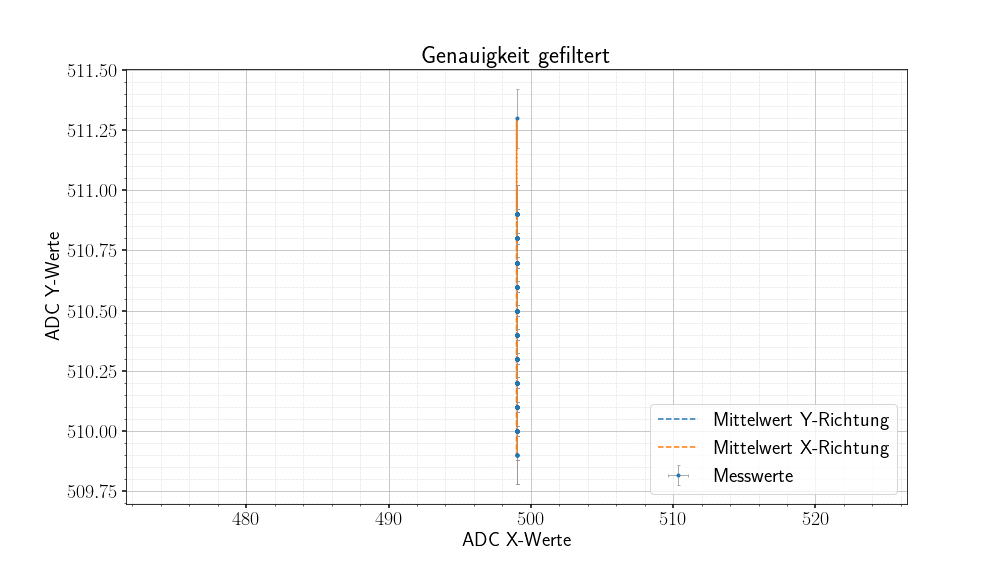
\includegraphics[width=\linewidth]{fig/filtered.png}
    \caption{Darstellung der gefilterten Messreihe}
    \label{fig:filtered}
    \centering
    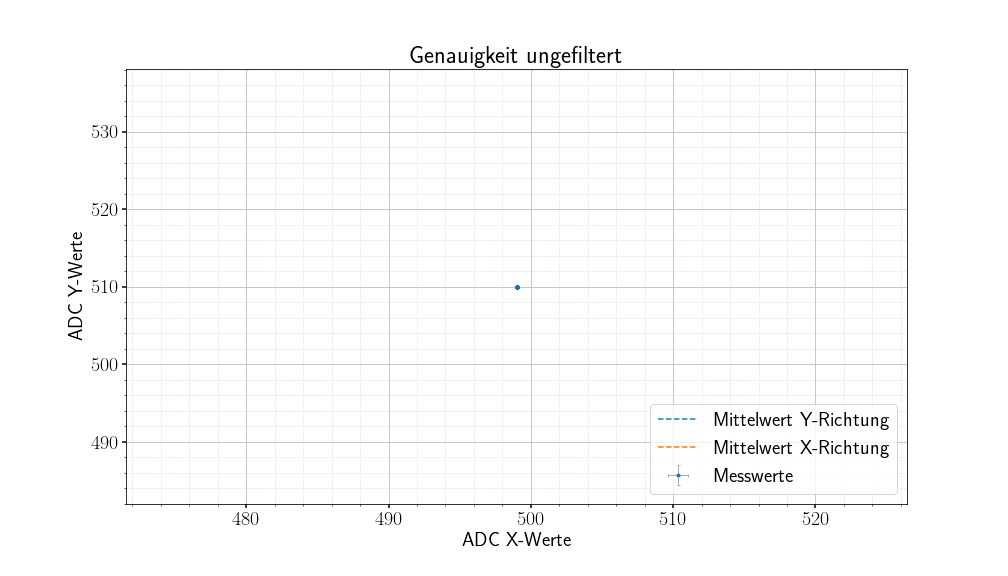
\includegraphics[width=\linewidth]{fig/unfiltered.png}
    \caption{Darstellung der ungefilterten Messreihe}
    \label{fig:unfiltered}
\end{figure}

\newpage

\section{Reproduzierbarkeit von Koordinaten}
\label{ab:wiederholung}
Um die Reproduzierbarkeit von Koordinaten zu untersuchen, wurde die Mitte des Touchscreen mehrmals berührt. Dabei wurden die ADC-Werte aufgezeichnet.
Ein Ausschnitt zu dieser Messreihe ist im Anhang auf Seite \pageref{tab:messwiederholung}. Die Messreihe wurde ebenfalls in einem Diagramm (Abb. \ref{fig:wiederholung} auf Seite \pageref{fig:wiederholung}) aufgetragen.

Die Auswertung der Messdaten sind in Tabelle \ref{tab:wiederholung} zu sehen. 
Diese zeigt, dass die Standardabweichung ähnlich der Auflösung. Dies lässt ebenfalls auf ein akkurat arbeitender Touchscreen schließen.


\begin{table}[ht!]
    \caption{Auswertung der Reproduzierbarkeit von Koordinaten}
    \begin{center}
        \begin{tabular}{ |c|c|c|c|c|c|c| }
          \hline  
         &\multicolumn{2}{c|}{Median}& \multicolumn{2}{c|}{Standardabweichung}&\multicolumn{2}{c|}{Varianz} \\ \hline
         Einheit    &(ADC)              &mm             &(ADC)          &mm             &(ADC)          &mm\\\hline
         x-Richtung & \SI{510,75}{}    & \SI{122,683}{}&\SI{0,894}{}   &\SI{0,215}{}   &\SI{0,8}{}     & \SI{0,192}{} \\  \hline
         y-Richtung & \SI{515,858}{}    & \SI{102,661}{}&\SI{1,159}{}   &\SI{0,231}{}   &\SI{1,3}{}     & \SI{0,259}{} \\ \hline  
        \end{tabular}
        \label{tab:wiederholung}
    \end{center}   
\end{table}


\begin{figure}[ht!]
    \centering
    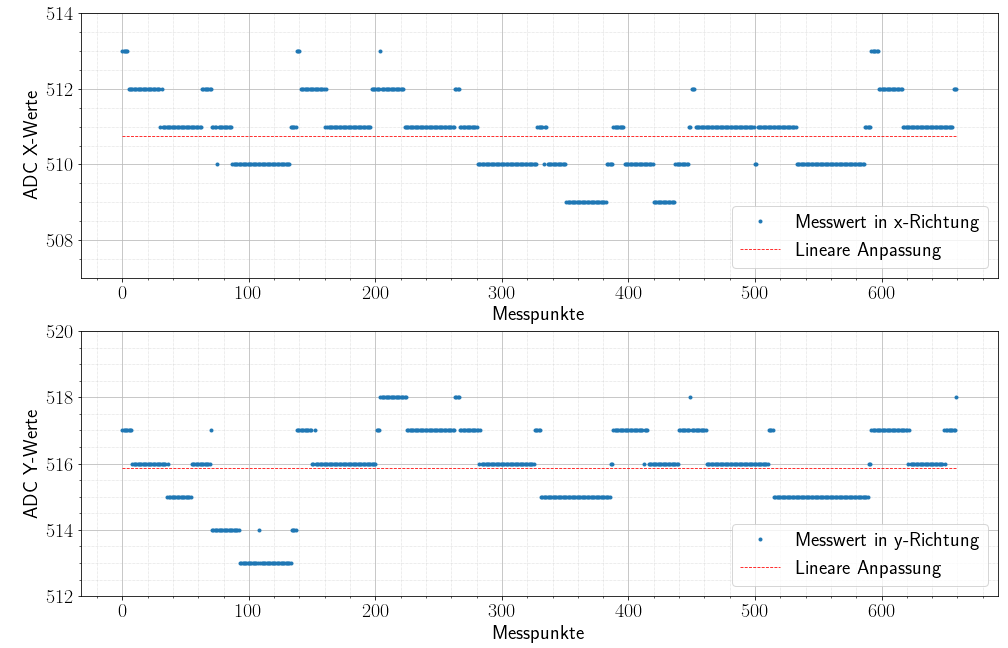
\includegraphics[width=\linewidth]{fig/wiederholung.png}
    \caption{Darstellung der Reproduzierbarkeit von Koordinaten}
    \label{fig:wiederholung}
\end{figure}
\section{Linearität in x- und y-Richtung}
\label{ab:linear}
Um eine Aussage über die Linearität des Touchscreens treffen zu können, wurden in x- und y-Richtung, auf dem Touchscreen alle \SI{10}{mm} eine Markierung gesetzt (siehe Abb. \ref{fig:messlinear}).

Die jeweilige Komponenten wurde anschließend jeweils über die physikalische Strecke in einem Diagramm dargestellt (siehe Abb. \ref{fig:xlinear} und Abb. \ref{fig:ylinear}). 
Die Messwerte wurden mittels einer linearen Anpassung anschließend ausgewertet (siehe Abb. \ref{fig:xfit} und Abb. \ref{fig:yfit}).

Das \(\chi^2\) gibt Auskunft darüber in welchem Maß Werte miteinander zusammenhängen. 
Je kleiner dieser Wert ist desto eher stimmt die Linearität überein. Bei der linearen Anpassung in x-Richtung wurde ein \(\chi^2\) von \(0,294\) ermittelt. Für die Linearität in y-Richtung wurde ein \(\chi^2\) von \(5,946\) ermittelt.

Bei der Untersuchung, der Linearität in y-Richtung, gibt es bei Abstand 40 mm ein Messpunkt der von der Messpunktewolke und der dazugehörigen linearen Anpassung abweicht. Dieser Messpunkt führt zu diesem größeren \(\chi^2\) als im Vergleich zur Messreihe  in x-Richtung.

Um Abschließend eine Aussage treffen zu können, ob diese Werte den Angaben des Datenblatts entsprechen (Anhang \ref{ds:touch}, Seite \pageref{ds:touch}), muss der Grenzwert der Chi-Quadrat-Verteilung mit den Werten der Linearen Anpassung verglichen werden.
Im Datenblatt wird eine Linearität von \SI{1,5}{\%} garantiert. In der Wertetabelle von \cite{papula} gibt es nur Grenzwerte für \SI{1}{\%} oder \SI{2,5}{\%}. Der gelistete Wert für zwei Freiheitsgrade und \SI{1}{\%} liegt bei 7,88.
Sowohl das \(\chi^2\) in x-Richtung wie auch in y-Richtung ist kleiner dieser Werte. Dies lässt darauf Schließen, dass dieser Touchscreen eine Linearität von unter \SI{1}{\%} aufweist.
\begin{figure}
    \begin{minipage}{0.49\linewidth}
        \centering
        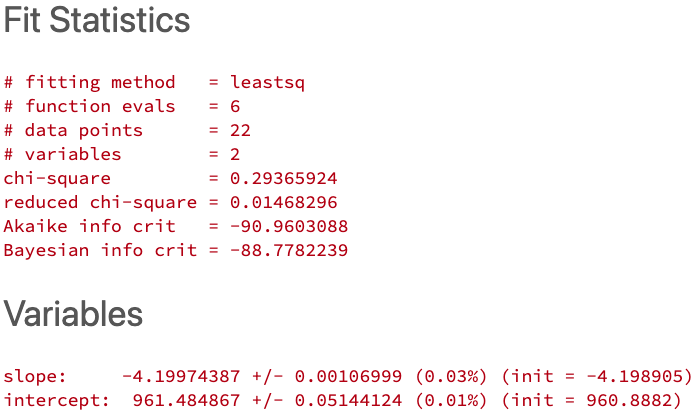
\includegraphics[width=\linewidth]{fig/xfit.png}
        \caption{Auswertung der Linearität in x-Richtung}
        \label{fig:xfit}
    \end{minipage}
    \begin{minipage}{0.49\linewidth}
        \centering
        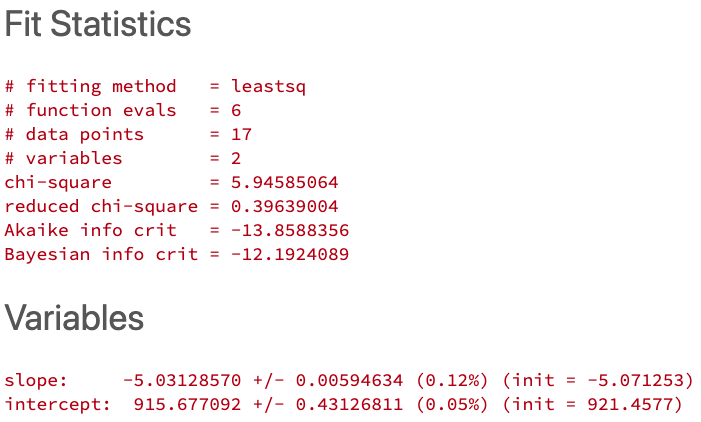
\includegraphics[width=\linewidth]{fig/yfit.png}
        \caption{Auswertung der Linearität in y-Richtung}
        \label{fig:yfit}
    \end{minipage}
\end{figure} 
\begin{figure}[ht!]
    \centering
    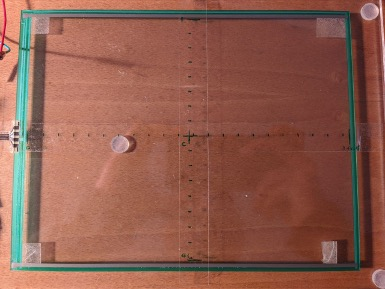
\includegraphics[width=0.6\linewidth]{fig/messlinear.jpg}
    \caption{Messaufbau für Linearität in x- und y-Richtung}
    \label{fig:messlinear}
\end{figure}

\begin{figure}[ht!]
    \centering
    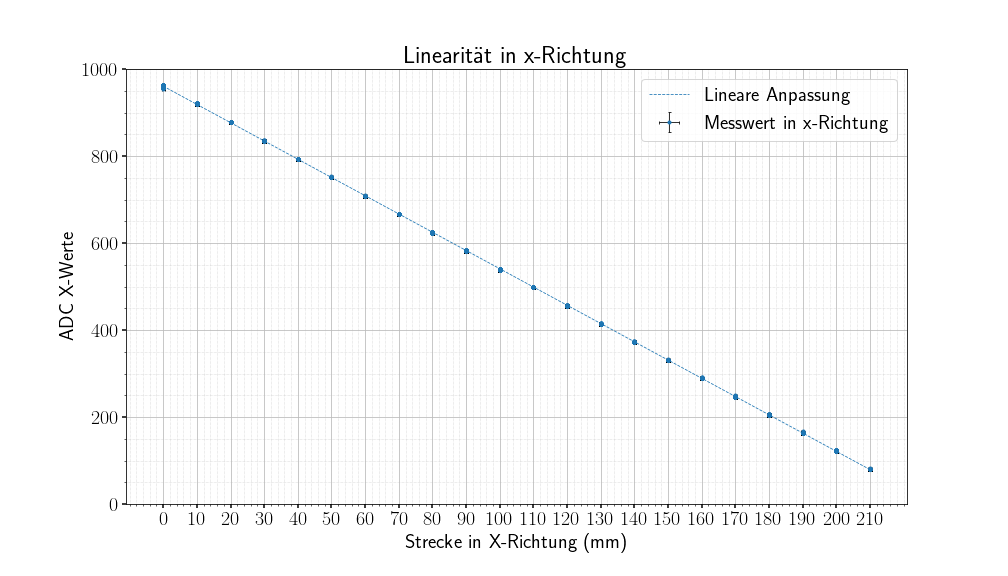
\includegraphics[width=\linewidth]{fig/8_linearitaet_x.png}
    \caption{}
    \label{fig:xlinear}
    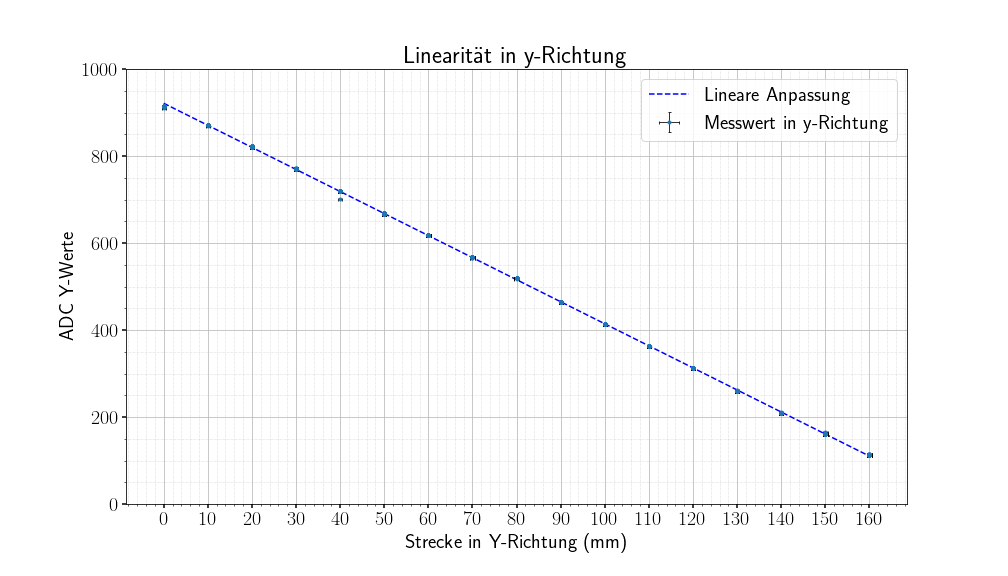
\includegraphics[width=\linewidth]{fig/8_linearitaet_y.png}
    \caption{}
    \label{fig:ylinear}
\end{figure}

    \chapter{Fazit}
\section{Qualität der Erkenntnisse}
Der uns ausgehändigte Touchscreen weißt zum einen eine ausgeprägte Genauigkeit wie auch Linearität auf. Es entspricht den Erwartungen und arbeitet zuverlässig.
Vor allem wenn ein Punkt übe längere Zeit bedrückt wird, weißt der Touchscreen eine hohe Genauigkeit auf. 
\section{Verbesserungsvorschläge}
  

    \appendix
    \chapter{Anhang}
        \section{Touchscreen}
            \label{ds:touch}
            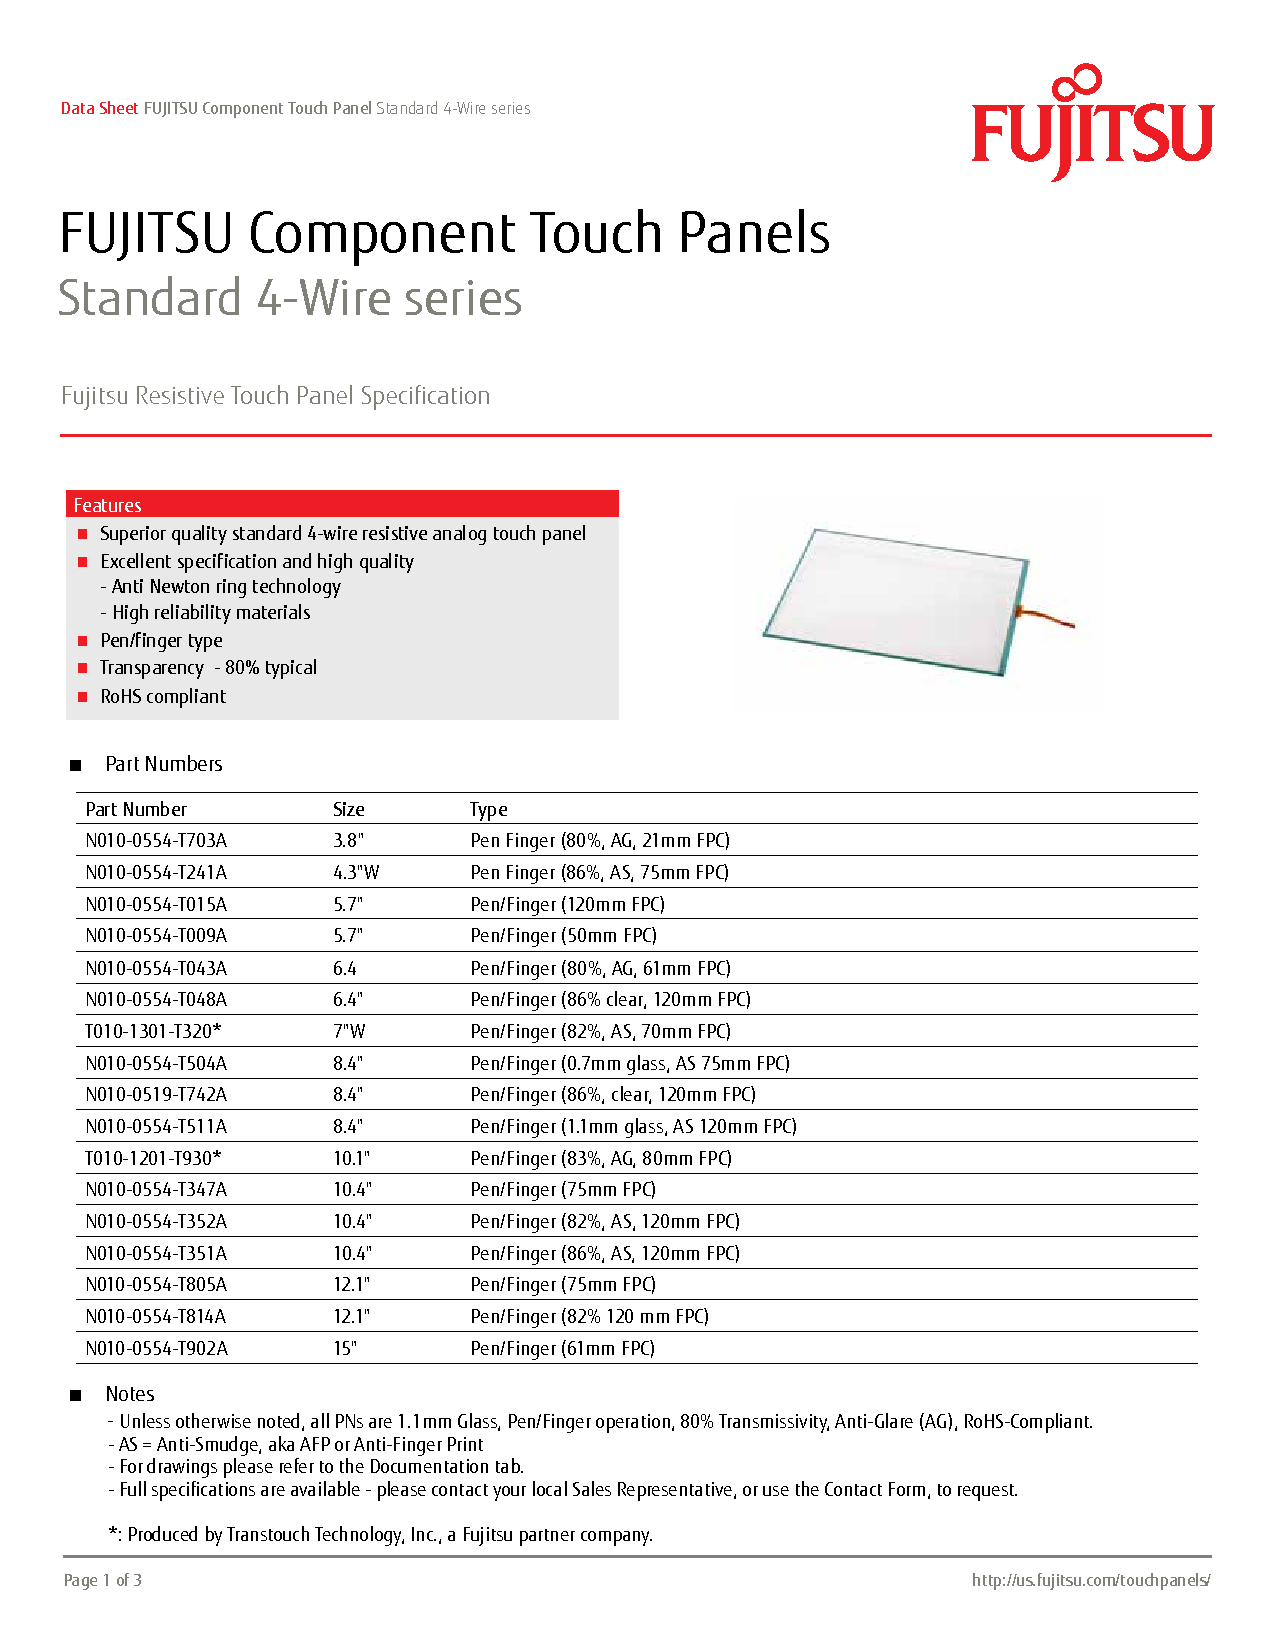
\includepdf[pages=-]{append/4_wire_standard_ds_rohs-10613.pdf}
        \section{Messdaten}
            \begin{table}[ht!]
                \begin{minipage}{0.49\linewidth}
                    \centering
                    \caption{Wertetabelle der gefilterten Genauigkeit}
                    \DTLsetseparator{;}
                    \DTLloaddb{scores}{messung/genauigkeitfiltered.csv}
                    \begin{tabular}{|c|c|}%
                        \hline x (ADC)& y (ADC)% specify table head
                        \DTLforeach{scores}{\x=x,\y=y}
                        {\\\hline\x & \y}\\
                        \hline
                    \end{tabular}
                    \label{tab:messgenaufilter}
                \end{minipage}
                \begin{minipage}{0.49\linewidth}
                    \centering
                    \caption{Wertetabelle der ungefilterten Genauigkeit}
                    \DTLsetseparator{;}
                    \DTLloaddb{score}{messung/genauigkeitunfiltered.csv}
                    \begin{tabular}{|c|c|}%
                        \hline x (ADC) & y (ADC)% specify table head
                        \DTLforeach{score}{\x=x,\y=y}
                        {\\\hline\x & \y}\\
                        \hline
                    \end{tabular}
                    \label{tab:messgenauunfilter}
                \end{minipage}
            \end{table}
\end{document}